% arara: xelatex
% arara: xelatex
% arara: xelatex


% options:
% thesis=B bachelor's thesis
% thesis=M master's thesis
% czech thesis in Czech language
% english thesis in English language
% hidelinks remove colour boxes around hyperlinks

\documentclass[thesis=B,english]{FITthesis}[2019/12/23]

%\usepackage[utf8]{inputenc} % LaTeX source encoded as UTF-8
% \usepackage[latin2]{inputenc} % LaTeX source encoded as ISO-8859-2
% \usepackage[cp1250]{inputenc} % LaTeX source encoded as Windows-1250

% \usepackage{subfig} %subfigures
% \usepackage{amsmath} %advanced maths
% \usepackage{amssymb} %additional math symbols

\usepackage{dirtree} %directory tree visualisation

% % list of acronyms
% \usepackage[acronym,nonumberlist,toc,numberedsection=autolabel]{glossaries}
% \iflanguage{czech}{\renewcommand*{\acronymname}{Seznam pou{\v z}it{\' y}ch zkratek}}{}
% \makeglossaries

% % % % % % % % % % % % % % % % % % % % % % % % % % % % % % 
% EDIT THIS
% % % % % % % % % % % % % % % % % % % % % % % % % % % % % % 

\department{Department of software engineering}
\title{Scala library for constructing statically typed PostgreSQL queries}
\authorGN{Petr} %author's given name/names
\authorFN{Hron} %author's surname
\author{Petr Hron} %author's name without academic degrees
\authorWithDegrees{Petr Hron} %author's name with academic degrees
\supervisor{Ing. Vojtěch Létal}
\acknowledgements{THANKS (remove entirely in case you do not with to thank anyone)}
\abstractEN{Summarize the contents and contribution of your work in a few sentences in English language.}
\abstractCS{V n{\v e}kolika v{\v e}t{\' a}ch shr{\v n}te obsah a p{\v r}{\' i}nos t{\' e}to pr{\' a}ce v {\v c}esk{\' e}m jazyce.}
\placeForDeclarationOfAuthenticity{Prague}
\keywordsCS{Scala, PostgreSQL, syntaktický strom, open source, validace během kompilace}
\keywordsEN{Scala, PostgreSQL, parse tree, open source, compile time validation}
\declarationOfAuthenticityOption{1} %select as appropriate, according to the desired license (integer 1-6)
% \website{http://site.example/thesis} %optional thesis URL


\begin{document}

% \newacronym{CVUT}{{\v C}VUT}{{\v C}esk{\' e} vysok{\' e} u{\v c}en{\' i} technick{\' e} v Praze}
% \newacronym{FIT}{FIT}{Fakulta informa{\v c}n{\' i}ch technologi{\' i}}

\setsecnumdepth{part}
\setsecnumdepth{all}
\chapter{Introduction}

\section{Motivation and goals}

Main goal of my work is to create Scala specific library to support constructing statically typed queries for Scala. This includes validation of queries and accessing internal PostgreSQL parse tree, which can be helpful for multiple different reasons....


\chapter{Technologies used}
\section{Scala}
\subsection{Introduction}
Scala belongs to the group of programming languages that can be compiled into Java byte code and run on a Java virtual machine (JVM). The major part, which makes it different from well-known Java, is the combination of applying a functional approach with an object-oriented paradigm. Together with the fact that Scala is similar to Java language itself, having the object-oriented style still present can ease up transition for programmers who are unfamiliar with the functional world.

\subsection{Static typing}

Besides the functional fundamentals, Scala is part of the family of statically typed languages, together with languages like C, C++, Java, or Haskell. Therefore, every single object in Scala has a type.

To make a job easier for the programmer, Scala uses a system known as type inference - automatic type detection. That allows faster coding, thanks to the fact you don’t have to worry about specifying every object’s type. However, providing types is always considered good practice, especially when we’re writing public API. Thanks to that, people who choose to use our code know what types of objects to expect. 

Since Scala compiler knows the types of the objects, it reveals many bugs during compilation. This is a great thing, because the sooner we can identify a bug, the easier it should be to fix it. 

\newpage
\section{PostgreSQL}
PostgreSQL is an ORDBMS, abbreviation for open source object-relational database management system.\cite{PostgreSQL} Origins date back to the year 1986, where the project then known as POSTGRES started as a reference to the older INGRES database. After 10 years it got renamed to PostgreSQL to clearly show its ability to work with SQL. 

Nowadays, it's used in many different projects. PostgreSQL popularity has been steadily rising in the last few years. Based on "Stack Overflow Annual Developer Survey"~\cite{Stackoverflow survey}, PostgreSQL currently sits at second place for the 'Most popular technology in the database category', right after the MySQL.

\subsection{Parse tree}
Postgres internally uses parse trees for processing SQL Queries. The whole parsing comprises multiple stages. First, the passed query, which is in the form of plain text, is transformed to tokens, using Unix tool "Flex". Next up the parser generator called "Bison" is called, which consists of multiple grammar rules and actions. Each action is executed whenever any of the rules are applied and together they are used to build the final parse tree.
\newline

\begin{figure}[h]
  \makebox[\textwidth]{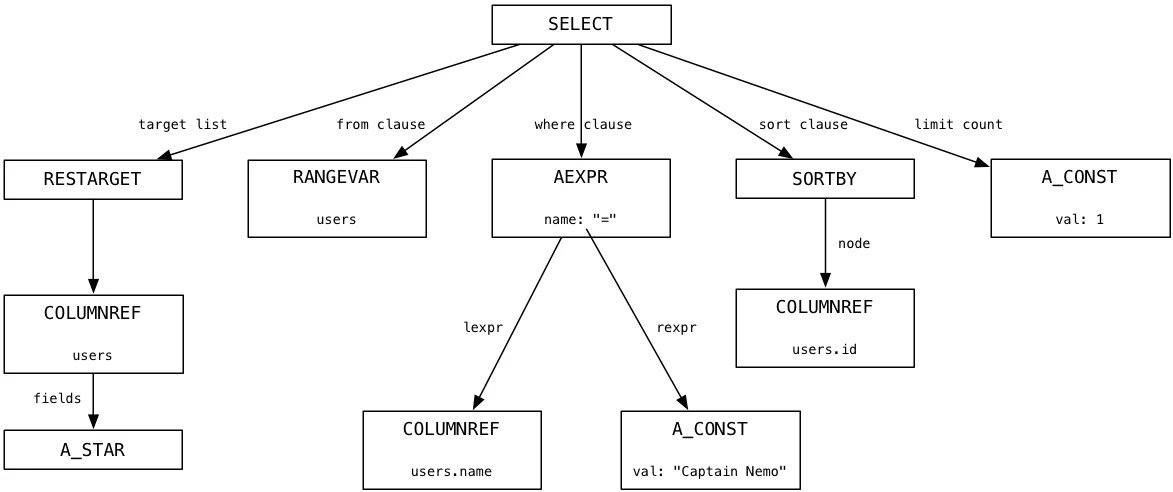
\includegraphics[width=\textwidth]{parse_tree.jpg}}
  \caption {Visualisation of parse tree for "SELECT * FROM users WHERE name = 'Captain Nemo' ORDER BY id ASC LIMIT 1'}
\end{figure}

\chapter{Existing options}
\section{Database libraries for Scala}
When we are working with databases in Java, we are most likely using JDBC, either directly or by wrappers like JPA or Hibernate. JDBC is available in Scala as well, by simply importing the `java.sql` API, you can create connections similarly as you would do in Java. But there are multiple existing libraries made for Scala, that ensure an easier way for the programmer to work with databases. Below I describe few selected libraries that were created for that specific reason.


\subsection{Quill}
Quill provides a Quoted Domain Specific Language (QDSL).~\cite{Quill} Its primary usage is to generate SQL queries, using only Scala code. Doing it this way Quill also provides type-safe queries, based on validation against defined database structure. The disadvantage of this approach is that the user can't validate generic queries without creating the case class database structure beforehand.

\subsection{Doobie}
Next up there is have Doobie, which is presented as \textit{"Doobie is a pure functional JDBC layer for Scala"}.~\cite{Doobie} In this library you can actually create pure SQL queries. The disadvantage is you have to have existing database and establish connection with it. That only allows run-time validation of queries.

\chapter{Realisation}

\section{Getting the SQL parse tree}

\subsection{libpg\_query}

\section{Connecting native code with java byte code}

\subsection{Java native interface}

\subsection{sbt-jni}

\section{Parsing JSON result from libpg\_query}

\subsection{JSON structure}

\subsection{Using `circe`}

\section{Deparsing back to SQL query}

\section{Scala custom interpolators}

\subsection{What are interpolators?}

\subsection{Implementation}

\subsection{`query` and `expr`}

\section{Scala macros}

\subsection{Implementation}

\subsection{Lifting}

\section{Combining interpolators and macros}

\subsection{Parameterized queries in PostgreSQL}

\subsection{Transforming syntax tree}

\section{Testing}
\section{Summary}

\section{Publishing library}

\setsecnumdepth{part}
\chapter{Conclusion}


\bibliographystyle{iso690}
\bibliography{mybibliographyfile}
\begin{thebibliography}{9}

\bibitem{PostgreSQL}
\textit {What Is PostgreSQL?} [online]. [cit. 2021-06-14]. Available from:
https://www.postgresql.org/docs/13/intro-whatis.html

\bibitem{Stackoverflow survey}
\textit {Stack Overflow Annual Developer Survey} [online]. [cit. 2021-06-13]. Available from: https://insights.stackoverflow.com/survey/2020\#technology-databases-all-respondents4

\bibitem{Quill} 
\textit {What is Quill?} [online]. [cit. 2021-04-25]. Available from: https://github.com/getquill/quill/
\bibitem{Doobie}
NORRIS, Rob. 
\textit {Doobie documentation} [online]. [cit. 2021-04-25]. Available from: https://tpolecat.github.io/doobie/
\bibitem{libpgquery}
FITTL, Lukas.
\textit {libpg\_query} [online]. [cit. 2021-04-25]. Available from:
https://github.com/pganalyze/libpg\_query
\bibitem{String interpolation}
SUERETH, Josh. 
\textit {String interpolation} [online]. [cit. 2021-04-25]. Available from: https://docs.scala-lang.org/overviews/core/string-interpolation.html
\bibitem{Def macros}
BURMAKO, Eugene. 
\textit {Def macros} [online]. [cit. 2021-04-25]. Available from: https://docs.scala-lang.org/overviews/macros/overview.html


\end{thebibliography}
\setsecnumdepth{all}
\appendix

\chapter{Acronyms}
% \printglossaries
\begin{description}
	\item[API] Application programming interface
	\item[JVM] Java virtual machine
\end{description}


\chapter{Contents of enclosed CD}

%change appropriately

\begin{figure}
	\dirtree{%
		.1 readme.txt\DTcomment{the file with CD contents description}.
		.1 exe\DTcomment{the directory with executables}.
		.1 src\DTcomment{the directory of source codes}.
		.2 wbdcm\DTcomment{implementation sources}.
		.2 thesis\DTcomment{the directory of \LaTeX{} source codes of the thesis}.
		.1 text\DTcomment{the thesis text directory}.
		.2 thesis.pdf\DTcomment{the thesis text in PDF format}.
		.2 thesis.ps\DTcomment{the thesis text in PS format}.
	}
\end{figure}

\end{document}
